\documentclass[]{article}
\usepackage{amsmath,amssymb,amsthm}
\usepackage[utf8]{inputenc}
\usepackage{lmodern}
%\usepackage{circuitikz}
\makeatletter
\@ifpackageloaded{tex4ht}{
    \def\pgfsysdriver{pgfsys-tex4ht.def}
}
\makeatother
\usepackage{pgfplots}
\usepackage{pgfplotstable}
\usepackage{pgf,tikz}
\usetikzlibrary{shapes,backgrounds,positioning,matrix,decorations}

\usepackage{siunitx}
\usepackage{python}
\usepackage{ifxetex,ifluatex}
\usepackage{listings}
% \usepackage[xindy,acronym,nomain,toc]{glossaries}
% \makeglossaries
%\usepackage[xindy]{imakeidx}
%\makeindex
\setlength{\parskip}{3mm}
\newtheorem{axiom}{Axiom}
\newtheorem{definition}{Definition}
\newtheorem{comment}{Comment}
\newtheorem{example}{Example}
\newtheorem{lemma}{Lemma}
\newtheorem{property}{Property}
\newtheorem{problem}{Problem}
\newtheorem{remark}{Remark}
\newtheorem{theorem}{Theorem}
\newtheorem{script}{Script}

\usepackage{fixltx2e} % provides \textsubscript
% use upquote if available, for straight quotes in verbatim environments
\IfFileExists{upquote.sty}{\usepackage{upquote}}{}
\ifnum 0\ifxetex 1\fi\ifluatex 1\fi=0 % if pdftex
  \usepackage[utf8]{inputenc}
\else % if luatex or xelatex
  \ifxetex
    \usepackage{mathspec}
    \usepackage{xltxtra,xunicode}
  \else
    \usepackage{fontspec}
  \fi
  \defaultfontfeatures{Mapping=tex-text,Scale=MatchLowercase}
  \newcommand{\euro}{€}
\fi
% use microtype if available
\IfFileExists{microtype.sty}{\usepackage{microtype}}{}
\ifxetex
  \usepackage[setpagesize=false, % page size defined by xetex
              unicode=false, % unicode breaks when used with xetex
              xetex]{hyperref}
\else
  \usepackage[unicode=true]{hyperref}
\fi
\hypersetup{breaklinks=true,
            bookmarks=true,
            pdfauthor={Dilawar Singh},
            pdftitle={Lecture 5, Question 2},
            colorlinks=true,
            citecolor=blue,
            urlcolor=blue,
            linkcolor=magenta,
            pdfborder={0 0 0}}
\urlstyle{same}  % don't use monospace font for urls
\setlength{\parindent}{0pt}
\setlength{\parskip}{6pt plus 2pt minus 1pt}
\setlength{\emergencystretch}{3em}  % prevent overfull lines
\setcounter{secnumdepth}{5}

\title{Lecture 5, Question 2}
\author{Dilawar Singh}
\date{\today}
\usepackage[margin=15mm]{geometry}

\begin{document}
\maketitle

\begin{quote}
You have two cells, each with the usual Na, K channels plus Ca channels
and Kca (Calcium-dependent K channels). One cell fires in bursts. The
other fires in an accommodating manner, that is fast at the beginning of
a current pulse, but slow towards the end. Draw calcium levels in the
two cases to explain how this happens.
\end{quote}

In both cells, roughly equal amount of Calcium should come it at each
action potential. Since both cells have different firing pattern,
$K_{Ca}$ channels must be different in both cells.

In accomodating cells, at each action potential if $x$ amount of Ca
enters the cell, less than $x$ amount of Ca goes out the cell before
next stimulus arrives, i.e.~we add some Ca into cell at each action
potential. This accumulating Ca opens up $K_{Ca}$ delaying the onset of
next action potential. This situation is shown in figure \ref{fig:1}.

In non-accommodating cells, if $x$ Ca enters the cell when it fires the
action potential, it goes out quickly enough. In short, Ca levels
remains fixed at certain level in cell. A typical case is shown in
figure \ref{fig:1}.

\begin{figure}[ht!]
\begin{center}
    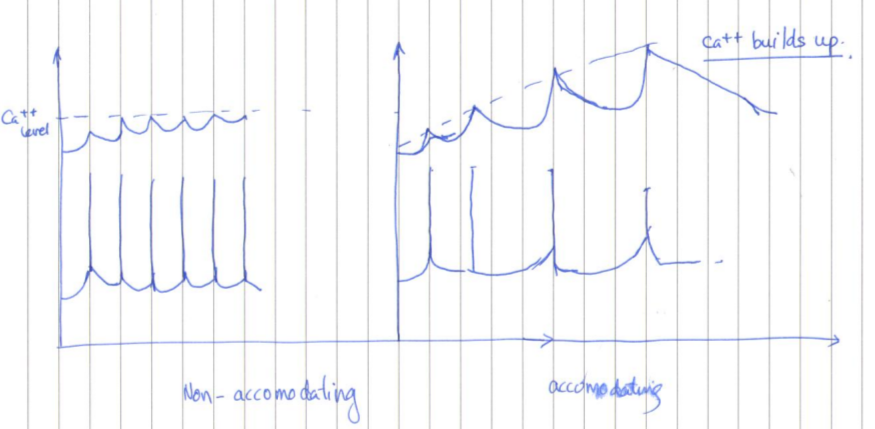
\includegraphics[width=1\textwidth]{scan.png}
\end{center}
\caption{}
\label{fig:1}
\end{figure}

\end{document}
